\chapter{Methodology and Design Process}

This chapter contains the design of the application architecture and scanning methodology. It explains the active studies finalized to the goal of the project.

\section{Standards and regulations}

This section provides an overview of the most relevant standards and regulations for the context of the internship's research, focusing on the industrial sector and the required goals; in particular, we detail more about \textit{IEC 62443}, \textit{ISO 27001}, \textit{NIS 2} and \textit{CRA}.

\subsection{IEC 62443}
\label{sec:iec-62443}

The IEC 62443 provides guidelines, rules and definitions specifically crafted for Industrial Automation and Control Systems (IACS). It is more focused on the specific sector while ISO 27001 is more universal and open for interpretation depending on the company it applies to.

The market requires the IEC 62443 certification for the companies that are involved in the production of industrial devices, as it is a guarantee of the security of the product and the company itself.

The IEC 62443 is a set of standards drafted by the \textit{Internation Electrotechnical Commission} (IEC) and it is divided into four categories:~\cite{iec-62443-parts-understanding}
\begin{enumerate}
  \item \textbf{General}: it covers topics that are common to the entire series;
  \item \textbf{Policies and procedures}: focuses on methods and processes associated with IACS security;
  \item \textbf{System}: it covers the requirements for the secure development and integration of systems;
  \item \textbf{Component}: it covers the requirements for the secure development and integration of components, defined as final products.
\end{enumerate}

\begin{figure}[ht]
  \centering
  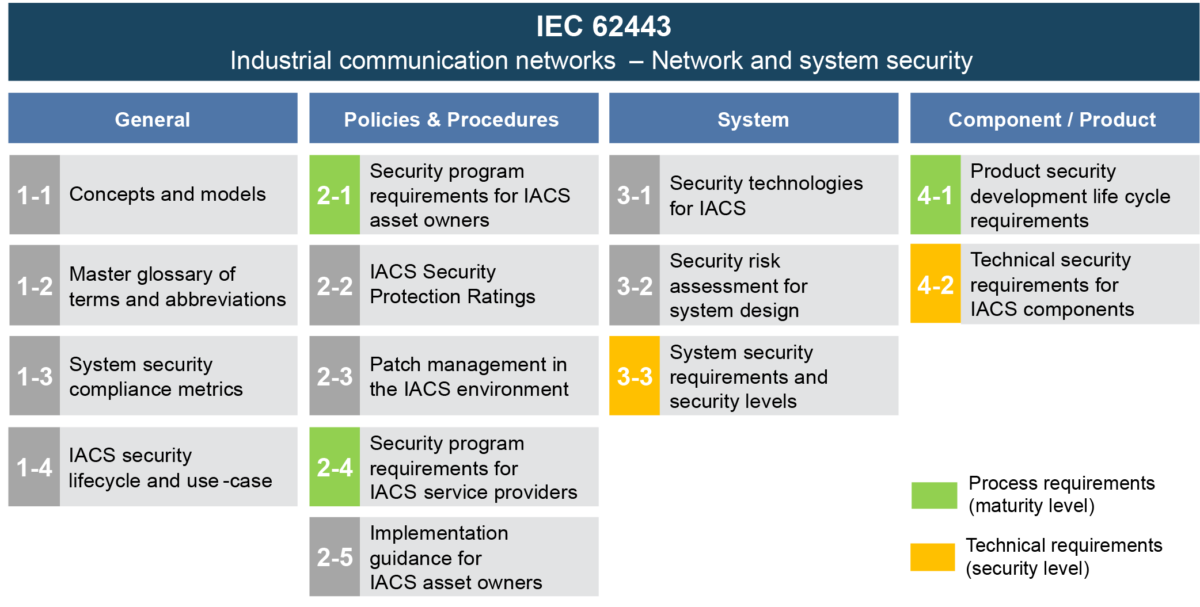
\includegraphics[width=0.9\textwidth]{chapters/04/assets/iec62443.png}
  \caption[IEC 62443 Parts and Sections. Image by Mohamed Wassef O.]{IEC 62443 Parts and Sections. Image by Mohamed Wassef O. on \url{https://www.linkedin.com/pulse/power-iec-62443-safeguarding-industrial-automation-othmani-gsrde}}
  \label{fig:iec-62443}
\end{figure}

Each category is divided into several subcategories, corresponding to different subjects. IEC 62443 is a comprehensive standard that covers all the specific aspects starting from the product design up to the development.

In the context of the internship project we are involved in, since we are directly at the level of product design and component development and deployment, the relevant subcategories we are focusing on are \texttt{3-3} and \texttt{4-2}, respectively named \textit{System security requirements and security levels} and \textit{Technical security requirements for IACS components}.

\texttt{IEC 62443-3-3} and \texttt{4-2} categorize seven \textit{Foundational Requirements} (FR) each, expanded respectively into a series of \textit{System Requirements} (SR) and \textit{Component Requirements} (CR) that the company must meet to obtain the certification.

For example, a system requirement taken from the subcategory \textit{System security requirements and security levels} (\texttt{3-3}) is the one shown in~\cref{fig:iec62443_3-3_3_9}. We are going to explain it in detail.

The foundamental requirement is \textit{FR 3 - System integrity} and the the system requirement states the following:
\begin{mdframed}
  SR 3.9 - Protection of audit information: The control system shall protect audit information and audit tools (if present) from unauthorized access, modification and deletion.
\end{mdframed}\label{sr:3-3_3-9}

Log audits are essential for the prevention and detection of cyberattacks. When something happens, log audit can help to understand what happened, when and where it happened and who was involved. This is a fundamental requirement for the IEC 62443 certification.

For each requirement listed in the documentation, the standard also describes some potential rationale and supplemental guidance to help the company understand the requirement and how to implement it.

Each system or component requirement is associated with at most four \textit{Requirement Enhancements} (RE) that can be implemented to increase the \textit{Security Level} (SL) of the system or component.

A security level is a measure of the security of a system or component, which is eventually transmitted to the final client: it is a score indicating how much sofisticated the solution is to follow the requirement. The minimum applicable security level is 1, while the maximum is 4.~\cite{iec-62443-ixon-practical-guide}\\
It is possible to increase the score of the security level by applying more non-trivial solutions, that is a requirement enhancement. An enhancement to increase the security level from 3 to 4 is stated in \texttt{SR 3.9 RE 1}:
\begin{mdframed}
  SR 3.9 RE 1 - Audit records on write-once media: The control system shall provide the capability to produce audit records on hardware-enforced write-once media.
\end{mdframed}\label{sr:3-3_3-9_re1}

We would like to note that not every SR has exactly four REs; instead, it could need fewer solutions in order to increase its score. For instance, this is the case for SR 3.9 which has only one RE and the minimum applicable SL is level 2, as shown in~\cref{fig:iec62443_3-3_3_9}.

\begin{figure}[ht]
  \centering
  \fbox{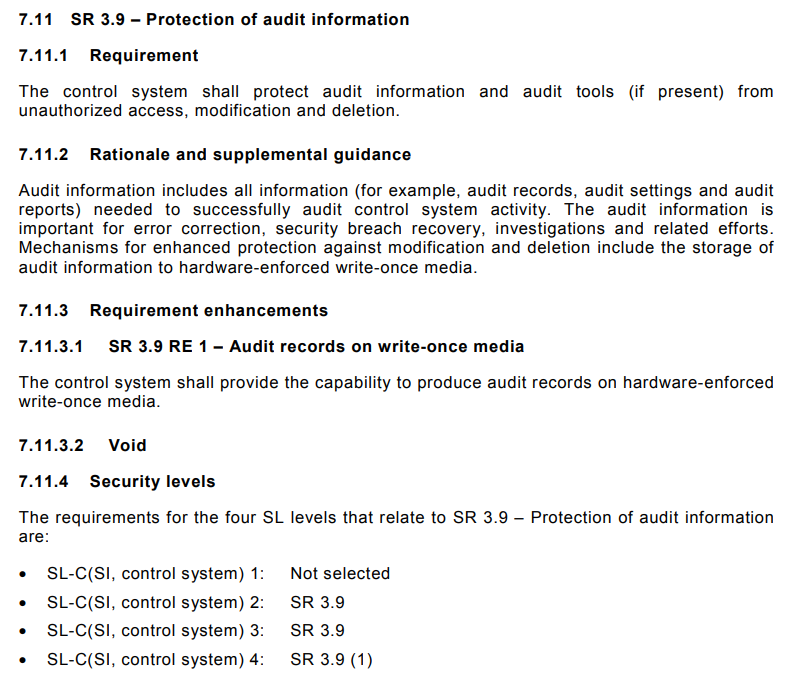
\includegraphics[width=1.0\textwidth]{chapters/04/assets/iec62443_3-3_3_9.png}}
  \caption[Snapshot of a IEC 62443-3-3 System Requirement]{Snapshot of a IEC 62443-3-3 System Requirement}
  \label{fig:iec62443_3-3_3_9}
\end{figure}

Moreover, sometimes the highest security level is not always the best solution or the most suitable for the company. Therefore, it is essential to evaluate the cost and the benefits of the solution before applying it.

At the system level, \texttt{IEC 62443-3-3} introduces security levels and corresponding requirements, offering a scalable framework to protect industrial systems. This part enables organizations to customize their security measures based on specific risk profiles and operational demands.

At the component level, \texttt{IEC 62443-4-1} lays the foundation for secure product development, emphasizing the critical importance of incorporating security measures right from the design phase. It encourages manufacturers to adopt a security-centric approach to product development, ensuring that components are fortified against cyber threats from the very beginning.\\
Moving from development to deployment, \texttt{IEC 62443-4-2} specifies the technical requirements for IACS components. It defines essential security capabilities such as robust authentication, encryption and intrusion detection, ensuring that each component reinforces the overall security of the system.~\cite{iec-62443-safeguarding-industrial-automation-linkedin}


\subsection{ISO/IEC 27001}

The ISO/IEC 27001 is a globally recognized standard addressed to companies of any size and from all sectors of activity with guidance for establishing, implementing, maintaining and continually improving an information security management system, which is a set of policies and procedures defining and managing controls that an organization needs to implement to ensure that it is sensibly protecting the confidentiality, availability and integrity of assets from threats and vulnerabilities. An information security management system that meets the requirements of ISO/IEC 27001 preserves the CIA triad and gives confidence to interested parties that risks are adequately managed.

Conformity with this standard means that an organization or business has put in place a system to manage risks related to the security of data owned or handled by the company and that this system respects all the best practices and principles enshrined in this International Standard.

It has been jointly published by the \textit{International Organization for Standardization} (ISO)~\cite{iso} and the \textit{International Electrotechnical Commission} (IEC)~\cite{iec}. The number indicates that it was published under the responsibility of Subcommittee 27 (on Information Security, Cybersecurity and Privacy Protection) of ISO's and IEC's Joint Technical Committee on Information Technology (ISO/IEC JTC 1).

It is widely used around the world; as per the ISO Survey 2022, over 70000 certificates were reported in 150 countries and from all economic sectors, ranging from agriculture through manufacturing to social services.~\cite{iso-27001}

\subsection{NIS Directive 2}
\label{sec:nis-directive-2}

The Network and Information Security (NIS) Directive is the first piece of EU-wide legislation on cybersecurity, drawn in 2016, and its specific aim was to achieve a high common level of cybersecurity across the Member States. To respond to the growing threats posed by digitalisation and the surge in cyber-attacks, the Commission has submitted a proposal to replace the NIS Directive and thereby strengthen the security requirements, address the security of supply chains, streamline reporting obligations and introduce more stringent supervisory measures and stricter enforcement requirements, including harmonised sanctions across the EU. NIS 2 entered into force on January 2023, and the Member States have until October 2024 to transpose its measures into national law.

The major key features of the updated directive are:~\cite{nis2-directive-faqs}
\begin{itemize}
  \item \textbf{Expanded scope}: NIS2 extends NIS scope to cover more sectors and industries. It applies to \textit{essential} and \textit{important} entities: NIS include energy (electricity, district heating and cooling, oil and gas), transport (air, rail, water and road), banking, health, pharmaceutical, water, digital infrastructure (internet exchange points, DNS providers, TLD name registries, cloud computing service providers, data centre service providers, content delivery networks), public administration and space. NIS2 include postal and courier services, waste management, chemicals, food, manufacturing of medical devices, computers and electronics, machinery equipment, motor vehicles and digital providers (online marketplaces, online search engines and social networking service platforms);
        % \\
        % Anyway, essential and important entities are deemed to be under the jurisdiction of the Member State where they provide their services;
  \item \textbf{Incident Reporting}: Companies must report significant cybersecurity incidents within 24 hours of detection, improving coordination between national cybersecurity authorities and helping mitigate the impact of attacks;
  \item \textbf{Fines and Penalties}: NIS2 introduces higher penalties for non-compliance, similar to the GDPR, with fines that could reach up to 2\% of an organization's total global turnover.
\end{itemize}

NIS 2 aims to enhance the resilience of the European digital market, ensuring the continuity of essential services even in the face of sophisticated cyberattacks.

\subsection{Cyber Resilience Act}

While the cybersecurity of providers of digital services is regulated at EU level by the NIS Directive 2, as analyzed in~\cref{sec:nis-directive-2}, the security of products with digital elements and software products is so far not subject to any comprehensive piece of EU regulation.~\cite{cra-eu}

Therefore, the European Commission proposed the Cyber Resilience Act in 2022; it has been approved in early 2024~\cite{cra-timelinel} and manufacturers have to place compliant products on the Union market by 2027, aiming to enhance the security of ICT products, services and processes.

It applies to products connected directly or indirectly to another device or network except for specific exclusions such as open-source software or services that are already covered by existing rules, which is the case for medical devices, aviation and cars. A non-exhaustive list of products that are in the scope of the CRA includes:~\cite{cra-overview}
\begin{itemize}
  \item \textbf{end devices}: laptops, smartphones, cameras, smart equipment, network equipment, Industrial Automation Control Systems (IACS);
  \item \textbf{software}: firmware, operating systems, applications;
  \item \textbf{components}: components like CPUs, video cards and libraries;
\end{itemize}

% With all being said, we now move to the next chapter, where we discuss how the directives and the standards we have just analyzed are applied in the context of the company we are working with and the internship project we are involved in.

\section{How IEC 62443 has driven the design}
\label{sec:iec-62443-driven-design}

Recalling~\cref{sec:iec-62443}, the IEC 62443 standard provides a comprehensive framework for securing industrial control systems and operational technology networks. In order to perform a step towards the certification of the devices with the standard, the scanning tool must cover at least the aspects of the standard.

First of all, our project is based on Component Requirement 6.2 as foundation:
\begin{mdframed}
  SR 6.2 - Continuous monitoring: The control system shall provide the capability to continuously monitor all security mechanism performance using commonly accepted security industry practices and recommendations to detect, characterize and report security breaches in a timely manner.
\end{mdframed}
With that said, our scanning tool will become the way to actively monitor the security of the devices and to report the results to the user for the company devices.

We did a case study on the standard documentation: for each of the requirements listed in the \texttt{3-3} and \texttt{4-2} documents we said:
\begin{mdframed}
  \textit{\textless\textless Can we implement a check for this requirement in such a way to make the user able to fix the potential issue by himself?\textgreater\textgreater}
\end{mdframed}\label{stm:check-}
We identified in the user that has a management account on the device, whom can interact on the system settings. The goal was to make the final customer able to fix the reported weaknesses in complete autonomy, by tweaking the settings and configuration of the device or eventually by updating the operative system.

\cref{fig:iec62443-findings-3_3} and~\cref{fig:iec62443-findings-4_2} show the findings of the case-study. The table is divided into four columns: the first one is the requirement title, the second one is the description, the third states whether we believe that it satisfies with our statement and the fourth one contains some notes about the possible implementation.

We already filtered the requirements that we believe relevant for the scanning tool, and we are going to evaluate them depending on the previous statement.

\begin{figure}[ht]
  \centering
  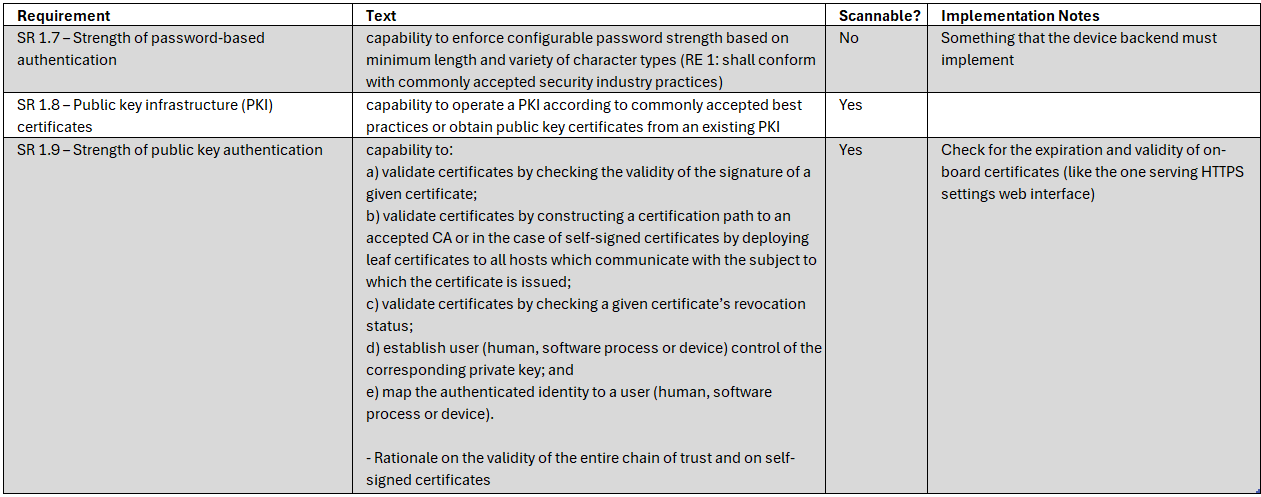
\includegraphics[width=1.0\textwidth]{chapters/04/assets/iec62443-findings-3_3}
  \caption{IEC 62443 \texttt{3-3} chosen requirements}
  \label{fig:iec62443-findings-3_3}
\end{figure}

\begin{figure}[ht]
  \centering
  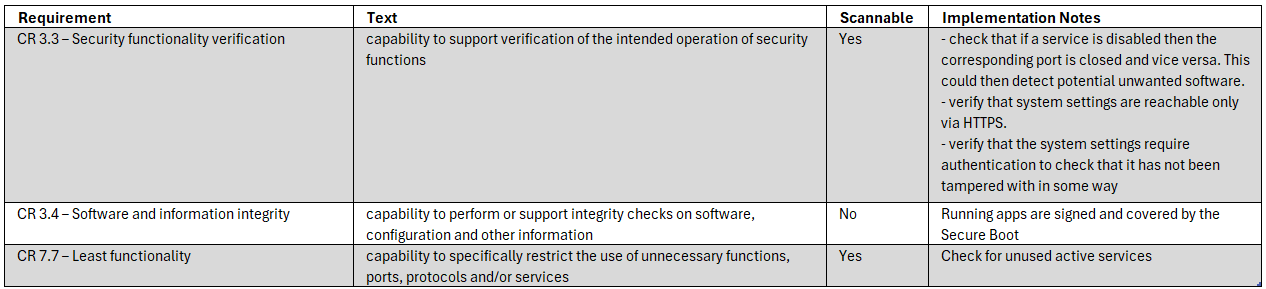
\includegraphics[width=1.0\textwidth]{chapters/04/assets/iec62443-findings-4_2}
  \caption{IEC 62443 \texttt{4-2} chosen requirements}
  \label{fig:iec62443-findings-4_2}
\end{figure}

To better explain our choices and motivations, we now take into account \textit{SR 1.9 - Strength of public key authentication} requirement. The requirement states that there must be the capability to enforce the validity of the used certificates by checking the signature, the expiration date and the revocation status. We believe that this is a check that we should implement in the scanning tool because the user can fix the issue by itself by renewing the certificate, or by changing the certificate authority if needed. The implementation could be done by retrieving the certificate from the device and then checking the signature, the expiration date and the revocation status. If the certificate is self-signed, the tool could suggest the user to replace it with another certificate signed by a trusted certificate authority.

On the other hand, let's consider \textit{SR 1.7 - Strength of password-based authentication}. The requirement states that the password must have a minimum length and a variety of different character types, but if the system could let the user set an invalid password, the tool cannot enforce that requirement because it could only suggest to change the password accordingly, without the possibility to enforce it. Therefore, the issue should be reported to the development team, which should implement a password policy, release a software update and the user should be then forced to change the password at the next login. In this specific case, we believe that the burden of checking and integrating this functionality, required by the standard, should be carried out separately from the execution of the tool by the end customer.

With this approach, we have identified the checks that the scanning tool should cover and we have included them in the backlog of the project.

\section{Backlog stories}

We have a backlog of stories for the scanning tool. Therefore, we drafted a new epic on the board and we filled it with the stories that we thought were needed to develop the tool.

We considered each story as an independent task that could be developed and tested in a short time, usually in a week. So, we split the epic into small stories, each one with a title, a description and a priority.

We started from the basis of a software, so the first stories were about the setup of the project and the thinking about the working architecture, the required parameters and the output formatting of the CLI. We want to keep the functioning of the tool as simple as possible and as much universal and reusable as possible. As a reference, we took inspiration by the help pages of some common software like \texttt{npm}, the NodeJS package manager, or \texttt{curl}, the tool to perform network requests directly on the terminal. Therefore, we sketched out the manual help page to have an overview of the commands and the options that the user could use.

At first glance, we decided to implement the following flow: the user runs the tool with the \texttt{scan} command, then the tool retrieves the device settings and the network status, then it performs the checks and finally it outputs the results to the console. The user can otherwise choose to save the output as an external file. The flag \texttt{--verbose} can be used to print more information about the checks and the results. The flag \texttt{--help} can be used to print the manual page or to print the documentation for a specific command.

The scan with no further options should perform all the checks that the tool can do as a default option, while the user can choose to perform only a subset of the checks by opting in using the \texttt{--list} flag. The list of the available checks is available by issuing the \texttt{list} command.

\noindent\begin{minipage}{\linewidth}
  \vspace{0.5cm}
  \begin{lstlisting}[caption={Man page}]
$ ./scantool
Industrial Security Scanning

Usage:
  scantool [command]

Available Commands:
  completion  Generate the autocompletion script for the specified shell
  help        Help about any command
  list        Show all the available scans
  scan        Start the device scan (options available typing `scan --help`)
  version     Print the version number

Flags:
  -h, --help      help for scantool
  --verbose       Log developer messages on stdout
  -v, --version   version for scantool
\end{lstlisting}
\end{minipage}

Moreover, we thought that the tool should be able to perform a scan in every network condition, to not exclude a priori a customer with an offline configuration or with a network that does not allow outgoing connections. Therefore, we decided to implement two different modes: the online mode where the tool can reach the cloud to determine the latest available version of the software and the offline mode where the tool cannot reach the cloud and has to rely on the local timestamp supplied by some of the software and libraries. The choice of the mode is automatic. \\
From the board side, for each of the checks that the tool should perform, we put at least two different stories, respectively one for the online mode and one for the offline mode.

Then, we sketched out the stories about the checks to perform, starting from those extracted from the IEC 62443 standard, as explained in~\cref{sec:iec-62443-driven-design}, but also adding some other checks that we thought needed to be performed. We also added some stories about the cross-compilation of the tool, the logging library to use and the CLI library to use.

At this point, we have a rich backlog of stories that we can work on and that we can prioritize according to the needs of the company.

The following list shows the stories that we have drafted for the scanning tool at the beginning of the project:
\begin{itemize}
  \item Choose a CLI library
  \item Choose a logging library
  \item Parse input parameters and output
  \item Split flow into offline and online usage
  \item Check correct time
  \item JSON output
  \item Cross build script
  \item Scan OS version - date based
  \item Scan OS version - version based
  \item Default BSP user credentials
  \item Default BSP admin credentials
  \item Scan SSH port
  \item Check VNC credentials
  \item Check certificate expiration
  \item Verbose flag
  \item Add YAML report formatter
\end{itemize}

The list is not exhaustive and it is subject to changes during the development of the tool. It is ranked by a first look at the priority of the stories, but the priority can change during the advancement of the project.

\section{Choosing the libraries}

Starting from scratch, we have to take care as first point of some utility libraries that we can use to draft the basis to develop the tool: we have to choose a CLI library to interact with and parse the command-line arguments, and a logging library to show the debug messages on the console or in another location.

\subsection{CLI library}

For the CLI parameters parsing we compared a library called \textit{urfave/cli/v2}\footnote{\url{https://github.com/urfave/cli}} (\texttt{v2.27.1}) and another one called \textit{spf13/cobra}\footnote{\url{https://github.com/spf13/cobra}} (\texttt{v1.8.0}). Data and evaluation refers to March 2024.

Both libraries have been recommended by the supervisor, and they are both widely used in the Go community. The evaluation between the two libraries is based on the features that they offer, the ease of use and the community support. In particular, we are interested in the ability to define flags and arguments, the ability to define commands and subcommands, the complexity of having a help page or the version of the tool.\\
Flags and arguments are the parameters that the user can pass to the tool to modify its behaviour, while commands are the different actions that the tool can perform. For example, the \texttt{scan} command is a command, while \texttt{--verbose} is a flag. Flag could be global, meaning that can be issued with every other command, or local, meaning that it has to be recognized only after a specified command or argument. A pattern to follow is \texttt{APPNAME COMMAND ARG --FLAG}. Finally, it's not obvious that a library supports the \textit{context} parameter, that is a way to pass data between the functions across the application.

\textit{urfave/cli/v2} is a package for building command line apps in Go. The package provides a way to define flags and arguments, and it also provides a way to define commands. The package has friendly documentation and it is actively maintained by the contributors. It is quick to define the actions for each flag or option. It supports the \textit{context} parameter. There is an upcoming major version \texttt{v3} in development, but it is not yet documented at all. The package has 21k stars on GitHub.

\textit{spf13/cobra} is a similar package for building command line apps in Go. The package provides a way to define flags and arguments, and it also provides a way to define commands. The documentation points directly to the source code, which is less friendly than the other package but anyway it is very rich and always updated. It supports the ability to deprecate a flag or a command with a custom message. It supports the \textit{context} parameter and an intelligent system of suggestions on typos, for example, if the user types a command that does not exist, the package suggests the most similar command. The package has 35k stars on GitHub and it is actively maintained.

We initialized an empty project and we tried to implement the same simple CLI with both libraries, one at time. The build size on the development laptop architecture with the first library was 4.8MB; with the second package was 5.1MB. The same working draft required 96 lines of code for the former and 110 lines of code for the latter.

In the end, we decided to use the \textit{spf13/cobra} because of the upcoming major version of \textit{cli/v2} which we do not know whether it will contain breaking changes or not, because the nice feature to deprecate an option, which could be useful given the youth of the project and possible future changes to the command-line interface and because of the capability to suggest the most similar command in case of a typo. The build size and the lines of code to get the same result are negligible for the use case of the tool.

\subsection{Log library}

The comparison for the logging library is between the standard library \textit{log}\footnote{\url{https://pkg.go.dev/log}} and another one called \textit{rs/zerolog}\footnote{\url{https://github.com/rs/zerolog}} (\texttt{v1.32.0}). Data and evaluation refer to April 2024.

The standard library \texttt{log} is the default logging package in Go. It provides a simple way to log messages with methods for formatting output. The package is easy to use and it is well documented. It supports the ability to log messages with different levels of severity, like \texttt{Info}, \texttt{Warning} and \texttt{Error}. The package is actively maintained by the contributors.

The \textit{rs/zerolog} lib, standing for \textit{Zero Allocation JSON Logger}, is another package for logging messages in Go. The package provides a way to log messages to the console or to a file. It also supports the different severity levels. The authors claim that the package is faster than other libraries because it does not allocate memory for the log messages~\cite{go-zerolog-benchmarks}. Furthermore, it implements pretty logging, a way to format the output in a human-readable way, the hooks to attach custom functions on an event, the \textit{context} integration and much more. It is actively maintained and it has 10k stars on GitHub.

With all being said, we decided to use the \textit{rs/zerolog} library because of the performance and the features that it offers. The package was also already used by the company in the cloud software, so it was a good choice to keep the same library for the scanning tool.

\section{Scanning tool web app}

The scanning tool is a command-line interface (CLI) application written in Go. The tool is designed to be run directly on the device, so it can be used by the user to check the configuration of the device and possibly receive suggestions on how to improve them. As an initial idea, the tool should be able to perform a scan of the device and output the results to the console. Thinking about the future, the scanning tool should be able to be run periodically and report the results to a central server, so the user can have a dashboard with the status of devices fleet.

The idea to consider is to make available the scanning tool through the applications store, so the user can enable the wider automation directly from the platform; the customer can create a campaign to verify the configuration of devices fleet from the same place and receive aggregated reports, with the goal to have a complete dashboard for the security status of the devices.
